\documentclass{ximera}

\title{Graphics, videos, and interactives}
\author{Bart Snapp and Jason Nowell}

\begin{document}
\begin{abstract}
  How to include graphics and other interactive content.
\end{abstract}
\maketitle
\label{xim:aGraphicsActivity}

\section{Including images}

In the last section, we showed you how to include images using
\verb|includegraphics|. However,
\textbf{the preferred method to include graphics is with TikZ.}
\begin{image}
  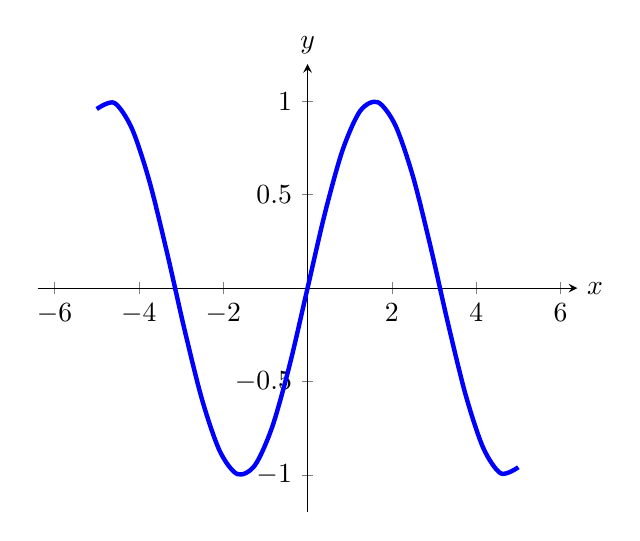
\begin{tikzpicture}
    \begin{axis}[
        xmin=-6.4,
        xmax=6.4,
        ymin=-1.2,
        ymax=1.2,
        axis lines=center,
        xlabel=$x$,
        ylabel=$y$,
        every axis y label/.style={at=(current axis.above
            origin),anchor=south},
        every axis x label/.style={at=(current axis.right of
            origin),anchor=west},
      ]
      \addplot [ultra thick, blue, smooth] {sin(deg(x))};
    \end{axis}
  \end{tikzpicture}
\end{image}
We can create the image above with the following code:
\begin{verbatim}
\begin{image}
  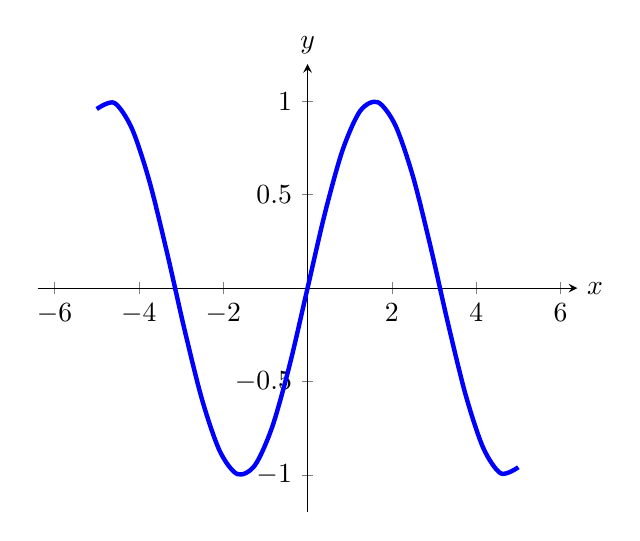
\begin{tikzpicture}
    \begin{axis}[
        xmin=-6.4,
        xmax=6.4,
        ymin=-1.2,
        ymax=1.2,
        axis lines=center,
        xlabel=$x$,
        ylabel=$y$,
        every axis y label/.style={at=(current axis.above origin),anchor=south},
        every axis x label/.style={at=(current axis.right of origin),anchor=west},
      ]
      \addplot [ultra thick, blue, smooth] {sin(deg(x))};
    \end{axis}
  \end{tikzpicture}
\end{image}
\end{verbatim}

\section{Videos}

We can embed YouTube Videos with the \verb|\youtube| command, for example,
\verb|\youtube{FvgF95i0_lw}| would embed the video into the page, like
this:
\begin{center}
  \youtube{FvgF95i0_lw}
\end{center}

\section{The graph command}

The easiest way to include an interactive graph is to use the
\verb|\graph| command. Unfortunately, the \verb|\graph| command
doesn't draw a graph in the PDF, rather, it states (in words) that a
graph is produced.
\[
  \graph{x^2}
\]
There are a number of options for the \verb|\graph| command, and you can find
out more WHERE?
Here are two examples. One with axis labels and a set window:

\[
  \graph[xAxisLabel="time", yAxisLabel="distance",xmin=0, xmax=10, ymin=0,
    ymax=10]{y=x^3}
\]

and another, piecewise function:
\[
  \graph{ \sin(x)\left\{x<0\right\}, 2x\left\{ x>=0 \right\} }
\]


\section{Desmos, Desmos3D, and Geogebra}

If you require further features from
\link[Desmos]{https://www.desmos.com/}, you can sign up for an account
and include your worksheets like this:

\begin{verbatim}
\begin{center}
\desmos{zwywds7med}{800}{600}
\end{center}
\end{verbatim}
\begin{center}
  \desmos{zwywds7med}{800}{600}
\end{center}

\link[Desmos3D]{https://www.desmos3d.com} and
\link[GeoGebra]{https://www.geogebra.org/} work in similar ways,
with:
\begin{center}
  \desmosThreeD{bb4exrhrl3}{800}{600}
\end{center}
generated by
\begin{verbatim}
\begin{center}
\desmosThreeD{bb4exrhrl3}{800}{600}
\end{center}
\end{verbatim}
and
\begin{center}
  \geogebra{XC3FXUdJ}{800}{600}%%https://www.geogebra.org/m/XC3FXUdJ
\end{center}
generated by:
\begin{verbatim}
\begin{center}
\geogebra{XC3FXUdJ}{800}{600}
\end{center}
\end{verbatim}

And remember the \hyperref[def:absolute_value]{definition of the absolute value}.

\end{document}
